\documentclass[12pt,a4paper]{article}

% Paquetes básicos
\usepackage[utf8]{inputenc}
\usepackage[T1]{fontenc}
\usepackage[spanish]{babel}
\usepackage{amsmath, amssymb}
\usepackage{siunitx} % Ángulos
\usepackage{graphicx}
\usepackage{float}
\usepackage{geometry}
\usepackage{xcolor}
\geometry{margin=2.5cm}
\usepackage{hyperref}
\usepackage{caption}
\usepackage{subcaption}
\usepackage{setspace}
\usepackage{multirow}
\usepackage{minted}  % Códigos
\usepackage{gensymb} % Grados: "°"
\usepackage[backend=biber, style=ieee]{biblatex}
\usepackage{csquotes}
\addbibresource{Bibliografía.bib}
\graphicspath{{Figuras/}}
\onehalfspacing
\hypersetup{
    colorlinks  = true,
    linkcolor   = blue,    
    citecolor   = blue,
    urlcolor    = blue,
    filecolor   = blue
}


\begin{document}       
\renewcommand{\figureautorefname}{Fig.}
\renewcommand{\tableautorefname}{Tab.}
\renewcommand{\equationautorefname}{Ec.}


% Carátula personalizada
\begin{titlepage}
    \centering
    
\includegraphics[width=0.7\textwidth]{Marvell Logo.png}\\[1.5cm]

    {\Large \textbf{PROGRAMA DE FORMACIÓN MARVELL} \\[0.5cm]}
    {\Large Comunicaciones Ópticas} \\[0.5cm]

    \rule{\textwidth}{0.5pt} \\[0.5cm]
    {\Large \textbf{Trabajo Práctico N°1: Análisis de Filtros  y Evaluación de Desempeño en Comunicaciones Digitales} \\[0.3cm]}
    \rule{\textwidth}{0.5pt} \\[1cm]
    
\begin{tabular}{l l}
    \textbf{Profesores:} & Francisco Rainero.\\
                         & Nestor Campos.\\
    \\[0.5cm]
    \textbf{Alumnos:} & Monja, Ernesto Joaquín (43.873.728)\\
                      & Zúñiga, Guillermo Rubén Darío (44.229.491)\\
\end{tabular} \\[5cm]

{\centering Año 2026 \par}

\end{titlepage}



% Índice
\tableofcontents
\newpage
\indent



\section{Introducción}                                                      \label{sec_1}
A lo largo de este informe se detalla el desarrollo y análisis de simulaciones orientadas a los fundamentos de las comunicaciones digitales de alta velocidad. El objetivo fundamental del trabajo es explorar y validar las técnicas de \textit{Pulse Shaping} necesarias para mitigar la Interferencia Inter-Símbolos (\textit{ISI}) y minimizar el ruido en un canal óptico. 

Para lograrlo, el estudio parte del diseño y caracterización de filtros clásicos como el Coseno Realzado (\textit{RC}) y su variante Raíz de Coseno Realzado (\textit{RRC}). Posteriormente, estos conceptos se integran en el modelado de transmisores elementales \textit{PAM-M} y sistemas completos de envolvente compleja \textit{QAM-M}, operando sobre canales afectados por Ruido Blanco Gaussiano Aditivo (\textit{AWGN}). A lo largo del documento, se evaluará el desempeño de los sistemas simulados en \textit{Python} mediante salidas gráficas y numéricas, incluyendo el análisis de Densidad Espectral de Potencia (\textit{PSD}), Diagramas de Ojo y de Constelaciones a la entrada del \textit{Slicer}, y curvas de Tasa de Error de Bit (\textit{BER}) contrastadas con modelos teóricos.



\section{Desarrollo}                                                        \label{sec_2}
\subsection{Diseño de Filtro \textit{Raised Cosine (RC)}}                   \label{sec_2.1}
El Coseno Realzado (\textit{RC}) es un filtro ampliamente utilizado en comunicaciones digitales debido a su capacidad para limitar el ancho de banda ($BW$) de la señal transmitida mitigando al mismo tiempo, la Interferencia Entre Símbolos (\textit{ISI}). Para su caracterización, se implementó una función en \textit{Python} \cite{b1} que genera la respuesta al impulso en base a la tasa de símbolos o \textit{Symbol Rate} (equivalente a $1/T$), la frecuencia de muestreo del filtro ($f_{s}$), el factor de \textit{Roll-Off} ($\beta$) y la cantidad de \textit{Taps} del filtro ($h_{taps}$).

A partir de este modelo, se analizaron las respuestas del filtro para un \textit{Symbol Rate} de $BR = 32 \ [GBd]$ y una frecuencia de muestreo $f_{s} = 4 \times BR$, variando el factor de \textit{Roll-Off} ($\beta \in \{0.0, 0.5, 1.0\}$). El comportamiento del filtro se evaluó tanto en el dominio del tiempo como en el de la frecuencia:
\begin{itemize}
    \item \underline{Análisis en el Dominio del Tiempo:} En la \autoref{fig:fig_1} se superponen las respuestas al impulso para los distintos valores de $\beta$.
    \begin{figure}[H]
        \centering
        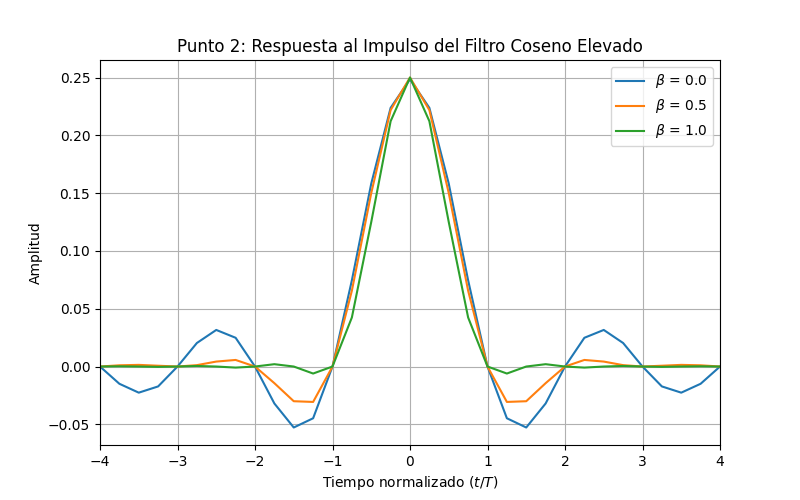
\includegraphics[width=1\linewidth]{Figura 1.png}
        \caption{Respuesta al Impulso del Filtro Coseno Realzado.} 
        \label{fig:fig_1}
    \end{figure}
    
    Al analizar la \autoref{fig:fig_1}, se observan las siguientes similitudes y diferencias:
    \begin{itemize}
        \item Todas las respuestas alcanzan su amplitud máxima en $t = 0$ y, fundamentalmente, presentan cruces por cero exactos en todos los múltiplos enteros del tiempo de símbolo ($t = \pm T, \pm 2T, \dots$). Esta es la condición de \textit{Nyquist} que garantiza que la interferencia entre símbolos (\textit{ISI}) sea nula en los instantes ideales de muestreo.
        
        \item La diferencia principal radica en la velocidad de decaimiento de los lóbulos laterales. Para un filtro ideal ($\beta = 0.0$), las oscilaciones decaen muy lentamente (función $sinc()$). A medida que se incrementa el valor de $\beta$ (como en la curva con $\beta = 1.0$), los lóbulos se atenúan con mucha mayor rapidez. En términos prácticos, un decaimiento rápido hace que el sistema sea más robusto frente a errores de sincronización en el receptor (\textit{Timing Jitter}), ya que los valores adyacentes al punto ideal de muestreo son cercanos a cero.
    \end{itemize}

    \item \underline{Análisis en el Dominio de la Frecuencia:} Mediante el uso de la Transformada Rápida de Fourier (\textit{FFT}), se obtuvo la magnitud de la respuesta en frecuencia de los filtros, la cual se presenta en la \autoref{fig:fig_2}. 
    \begin{figure}[H]
        \centering
        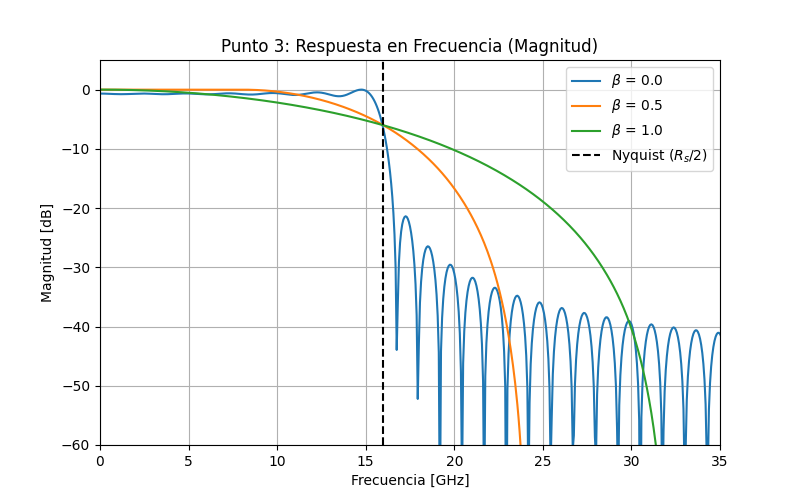
\includegraphics[width=1\linewidth]{Figura 2.png}
        \caption{Respuesta en Frecuencia (Magnitud).} 
        \label{fig:fig_2}
    \end{figure}
    De este espectro se desprenden las siguientes similitudes y diferencias:
    \begin{itemize}
        \item Todas las curvas presentan una magnitud constante en frecuencias bajas y cruzan el punto de atenuación de $-3 \ [dB]$ (mitad de potencia) exactamente en la misma frecuencia: la frecuencia de \textit{Nyquist}, equivalente a $R_{s}/2$ ($16 \ [GHz]$ para este caso).

        \item La distinción fundamental es el ancho de banda absoluto que ocupa cada filtro en el espectro. El ancho de banda total necesario ($BW$) crece linealmente con el exceso de ancho de banda $\beta$, según la relación teórica:
        \begin{equation}
            BW = \frac{BR}{2} (1 + \beta)
            \label{eq_1}
        \end{equation}
        
        Esto se evidencia claramente en la \autoref{fig:fig_2} ya que el filtro con $\beta = 0.0$ presenta un corte abrupto y ocupa el mínimo espectro teórico ($16 \ [GHz]$) y en contraparte, al aumentar el \textit{Roll-Off} a $\beta = 1.0$, el espectro se ensancha hasta ocupar el doble de ancho de banda ($32 \ [GHz]$).
    \end{itemize}
\end{itemize}

En síntesis se tiene que la selección del parámetro $\beta$ representa un compromiso de diseño directo: un mayor exceso de ancho de banda sacrifica eficiencia espectral para obtener un pulso en el tiempo con menor interferencia residual ante errores de muestreo.




\subsection{Diseño de Filtro \textit{Root-Raised Cosine (RRC)}}             \label{sec_2.2}
El filtro raíz coseno realzado (\textit{RRC}) es implementado en el transmisor y el receptor para lograr que la respuesta compuesta sea un filtro coseno realzado (\textit{RC}) ---ya que la convolución entre dos \textit{RRC} es un \textit{RC}--- y así eliminar la \textit{ISI} dentro del ancho de banda de trabajo. 

Se realizó un script de \textit{Python} \cite{b2} que genera distintos filtros \textit{RRC}, con $\beta$ como parámetro. En la \autoref{fig:fig_3} se observa la respuesta al impulso del \textit{RRC} según el $\beta$. Se puede ver que ninguno de los filtros cruza por cero en múltiplos de $T$, excepto cuando $\beta = 0$, que es cuando el \textit{RRC} se convierte en un $sinc$. Se concluye entonces que el \textit{RRC} no cumple con el criterio de \textit{Nyquist} por sí solo; sin embargo y como se mencionó anteriormente, la implementación de un \textit{RRC} en el transmisor y uno en el receptor, provoca que la señal ``vea'' un \textit{RC}. Por otro lado y al igual que en el \textit{RC}, la diferencia que genera el $\beta$ es la cantidad de muestras que se necesitan para sintetizar el filtro en su totalidad, observándose en la figura cómo un mayor \textit{Roll-off} implica una menor cantidad.
\begin{figure}[H]
    \centering
    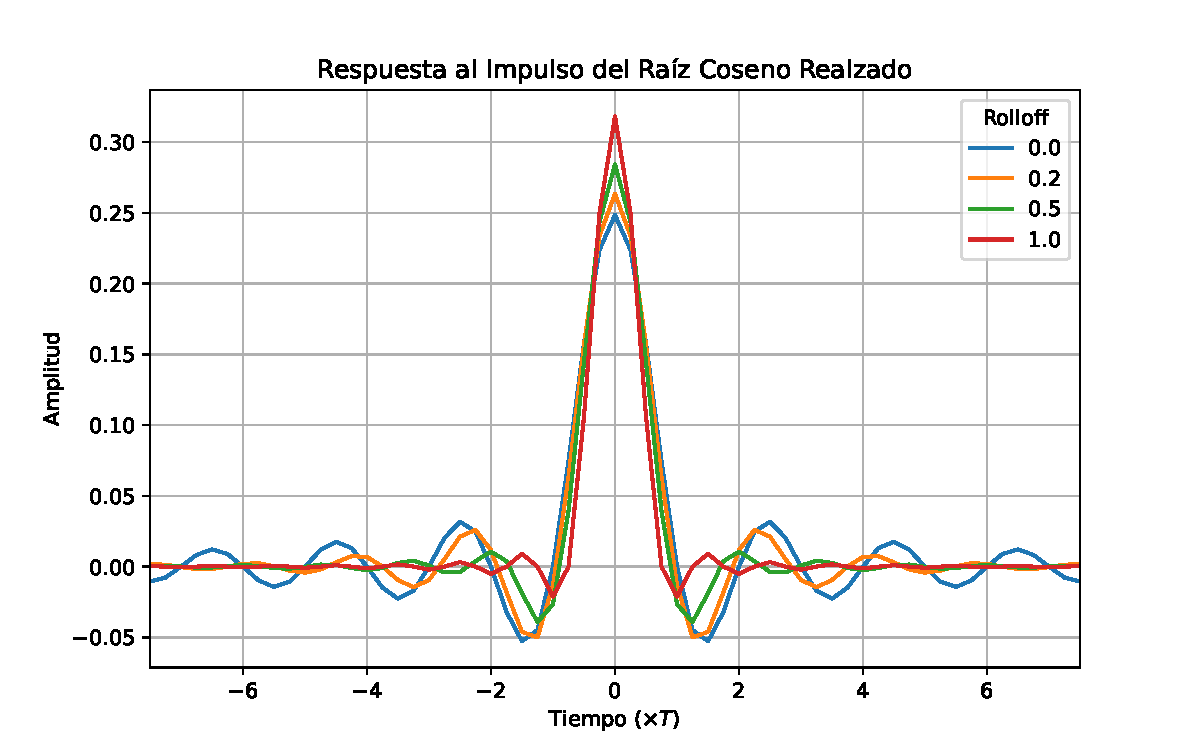
\includegraphics[width=0.8\linewidth]{Figura 3.pdf}
    \caption{Respuesta al impulso del Raíz Coseno Realzado según $\beta$.}
    \label{fig:fig_3}
\end{figure}

El ancho de banda del filtro también tiene un exceso determinado por el \textit{Roll-off}. Se comparó la respuesta en frecuencia con distintos $\beta$, con los resultados mostrados en la \autoref{fig:fig_4}.

Con $\beta$ próximo a 0, la respuesta en frecuencia es más estrecha y cercana al ideal de \textit{Nyquist}. Con $\beta$ creciente, el ancho de banda ocupado aumenta pero la frecuencia de corte también, mientras que en el \textit{RC} se mantiene constante en los $16 \ [GHz]$. Por otro lado, se observa que el nivel de atenuación fuera de la banda de paso disminuye para $\beta$ más pequeños; esto es porque la cola de la respuesta temporal no se termina de extinguir en la ventana temporal, generando componentes de alta frecuencia.
\begin{figure}[H]
    \centering
    \begin{minipage}{0.48\linewidth}
        \centering
        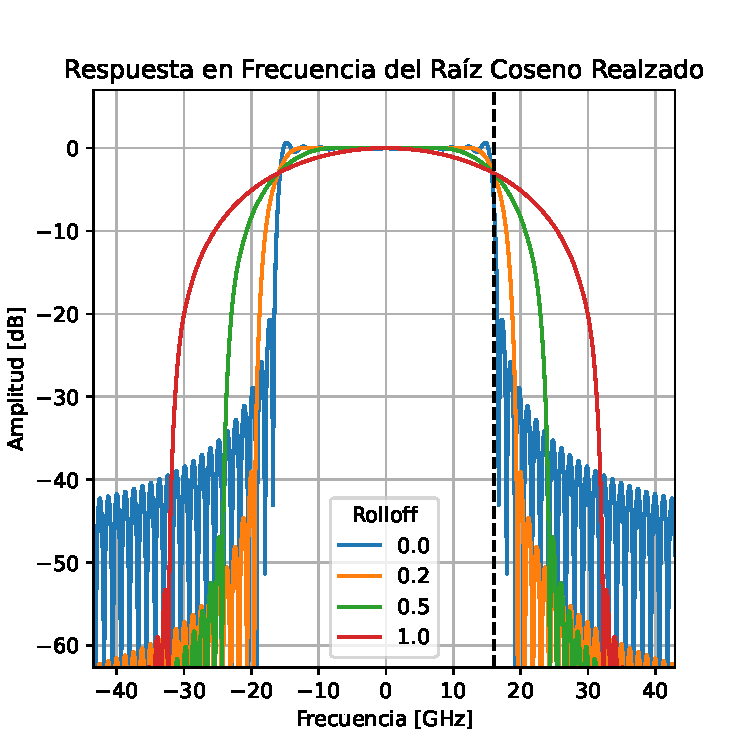
\includegraphics[width=1\linewidth]{Figura 4.1.pdf}
    \end{minipage}
    \hfill
    \begin{minipage}{0.48\linewidth}
        \centering
        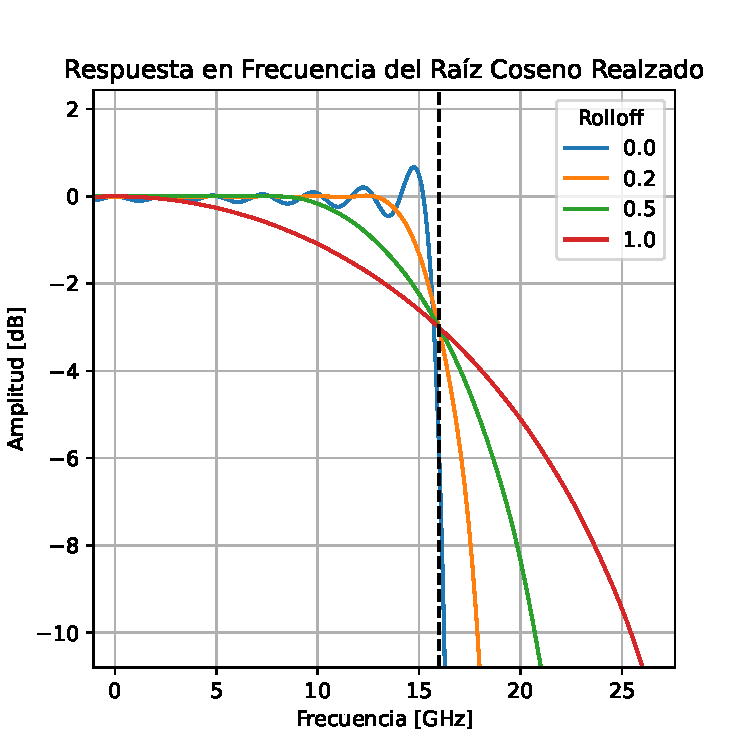
\includegraphics[width=1\linewidth]{Figura 4.2.pdf}
    \end{minipage}
    \caption{Respuesta en $[dB]$ del Raíz Coseno Realzado según $\beta$.}
    \label{fig:fig_4}
\end{figure}

A modo de comparación, se muestra la respuesta al impulso de un \textit{RRC} y un \textit{RC} en la \autoref{fig:fig_5}, donde se observa mejor cómo el \textit{RC} cruza por cero en múltiplos de $T$, mientras que el \textit{RRC} no lo hace. Se verifica también que la convolución de dos \textit{RRC} es efectivamente un \textit{RC}.
\begin{figure}[H]
    \centering
    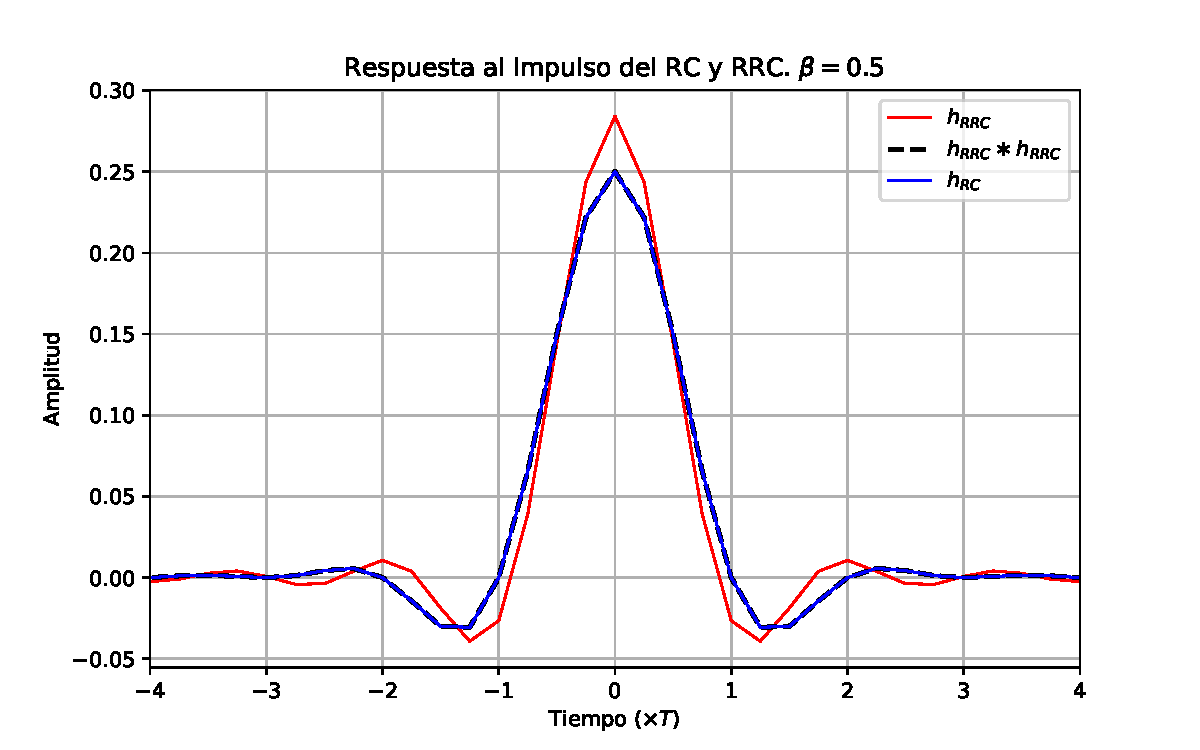
\includegraphics[width=0.75\linewidth]{Figura 5.pdf}
    \caption{Respuesta al impulso de un \textit{RRC} y un \textit{RC}. $\beta = 0.5$.}
    \label{fig:fig_5}
\end{figure}

La comparación en frecuencia se puede apreciar en la \autoref{fig:fig_6}. Se puede decir que el ancho de banda útil entre ambos es la misma al tener el mismo factor de \textit{Roll-Off}, sin embargo, en este caso se aprecia mejor la diferencia en la frecuencia de corte, donde en el \textit{RC} es de $16 \ [GHz]$ y en el \textit{RRC} es aproximadamente $19 \ [GHz]$. Además de que el \textit{RRC} presenta una atenuación diferente fuera de banda, cuya amplitud es del doble de la del \textit{RC}.
\begin{figure}[H]
    \centering
    \begin{minipage}{0.5\linewidth}
        \centering
        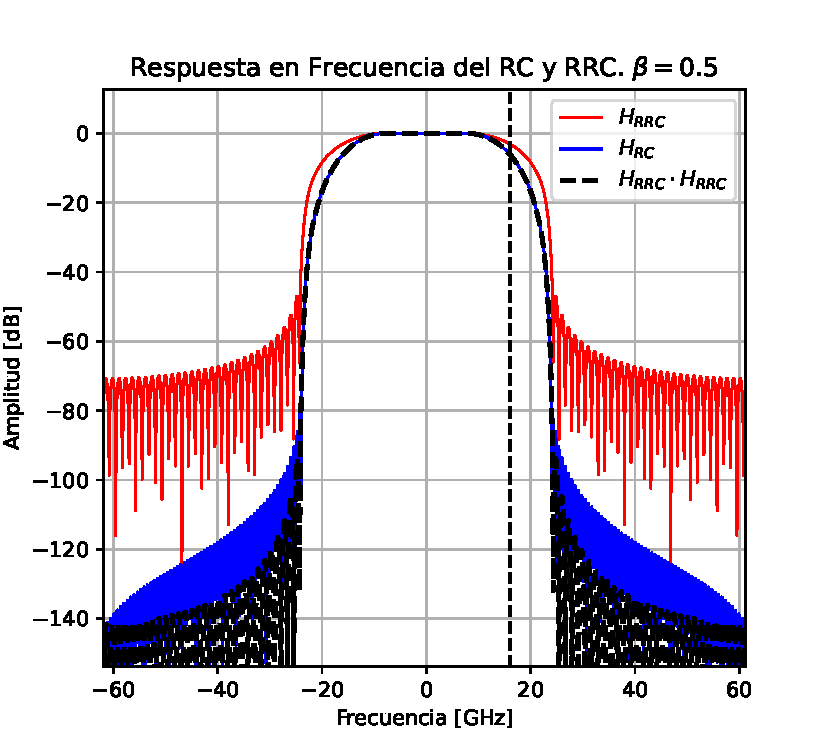
\includegraphics[width=0.8\linewidth]{Figura 6.1.pdf}
    \end{minipage}
    \hfill
    \begin{minipage}{0.46\linewidth}
        \centering
        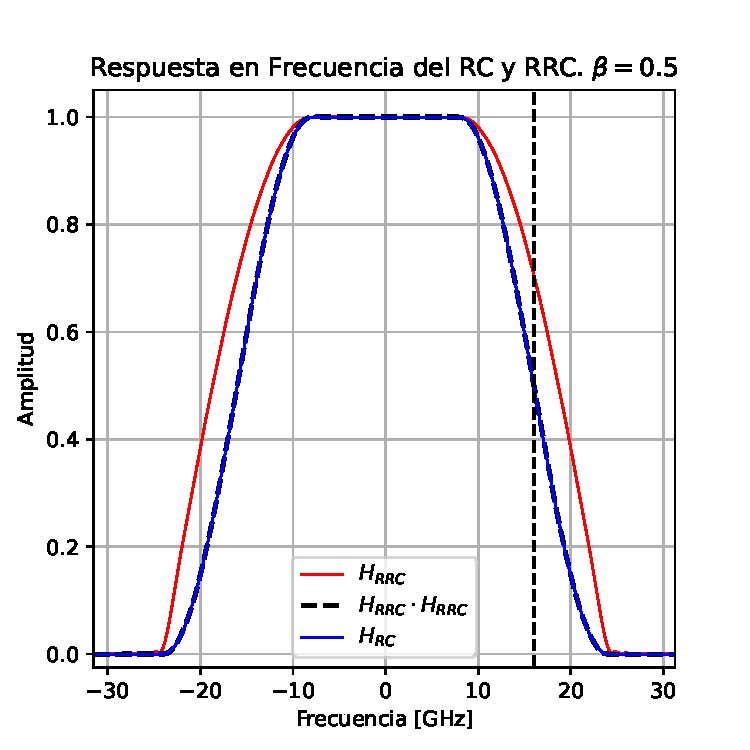
\includegraphics[width=0.8\linewidth]{Figura 6.2.pdf}
    \end{minipage}
    \caption{Respuesta en frecuencia de un \textit{RRC} y un \textit{RC}. $\beta = 0.5$.}
    \label{fig:fig_6}
\end{figure}




\subsection{Transmisión de Símbolos, Alineación Temporal y Conformación Espectral}  \label{sec_2.3}
Con el objetivo de evaluar el desempeño de los filtros estudiados en un escenario de transmisión, se implementó una cadena de transmisión básica. Se generó una secuencia de símbolos $a_{k}$ pertenecientes a un alfabeto discreto (modulación \textit{PAM-4}) operando a una tasa de $BR = 32 \ [GBd]$. Esta secuencia fue sometida a un proceso de sobre muestreo (insertando $N-1$ ceros entre cada símbolo, con $N = 4$) y posteriormente conformada mediante filtrado digital.


\subsubsection{Análisis en el Dominio del Tiempo: Interferencia Entre Símbolos (\textit{ISI})} \label{sec_2.3.1}
Para analizar el impacto del filtrado en la recuperación de la información, se superpusieron los instantes de transmisión ideal de los símbolos $a_{k}$ (representados mediante la función $stem$) con la señal analógica equivalente $s(t)$ a la salida del filtro, compensando previamente el retardo introducido por el mismo ($N_{taps}-1 / 2$).

Para esto, se realizó un script en \textit{Python} \cite{b3} el cual presenta como primera salida la \autoref{fig:fig_7}.
\begin{figure}[H]
    \centering
    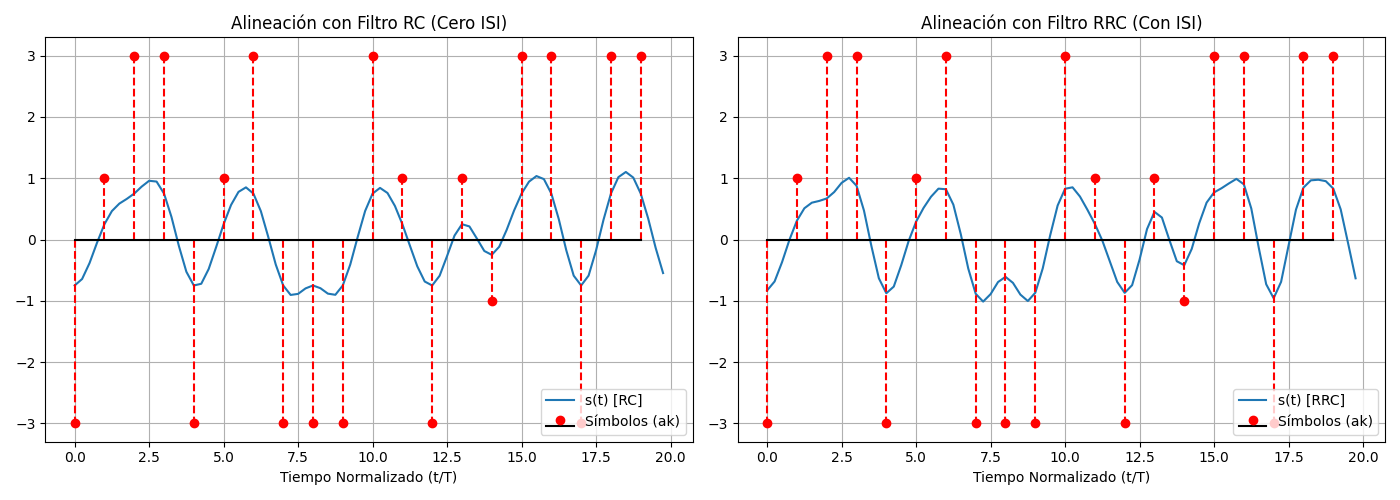
\includegraphics[width=0.9\linewidth]{Figura 7.png}
    \caption{Alineación de los Filtros \textit{RC} y \textit{RRC}.} 
    \label{fig:fig_7}
\end{figure}

Al observar los resultados utilizando el filtro Coseno Realzado (\textit{RC}) (ver la gráfica izquierda de la \autoref{fig:fig_7}), se verifica que en los instantes de muestreo $t = kT$, la señal $s(t)$ intersecta de manera exacta la amplitud de los símbolos transmitidos. Esto corrobora empíricamente que el filtro \textit{RC} cumple el criterio de \textit{Nyquist}, garantizando nula Interferencia Entre Símbolos (\textit{Zero-ISI}), lo que permitiría detectar los símbolos directamente a la salida del transmisor.

Por el contrario, al emplear el filtro Raíz de Coseno Realzado (\textit{RRC}) (ver la gráfica derecha de la \autoref{fig:fig_7}), se evidencia que la señal conformada no coincide con los símbolos $a_{k}$ en los instantes de muestreo ideales. A partir de esta señal $s(t)$ no es posible realizar una detección directa libre de errores, ya que el sistema presenta una fuerte presencia de \textit{ISI}. Este comportamiento es el esperado, dado que el filtro \textit{RRC} representa matemáticamente la raíz cuadrada de la respuesta de \textit{Nyquist}; para lograr la cancelación total de la interferencia, es imperativo implementar un segundo filtro \textit{RRC}, denominado también Filtro Apareado o \textit{Matched Filter} del Inglés en la etapa de recepción, cuya respuesta combinada $|H_{RRC}(\omega)|^2$ resulte en un Coseno Realzado puro.


\subsubsection{Análisis de la Densidad Espectral de Potencia (\textit{PSD})}         \label{sec_2.3.2}
Adicionalmente, se estudió el impacto espectral del proceso de conformación mediante la estimación de la Densidad Espectral de Potencia utilizando el método de \textit{Welch} tal como lo muestra la \autoref{fig:fig_8} del script de \textit{Python} \cite{b3}.
\begin{figure}[H]
    \centering
    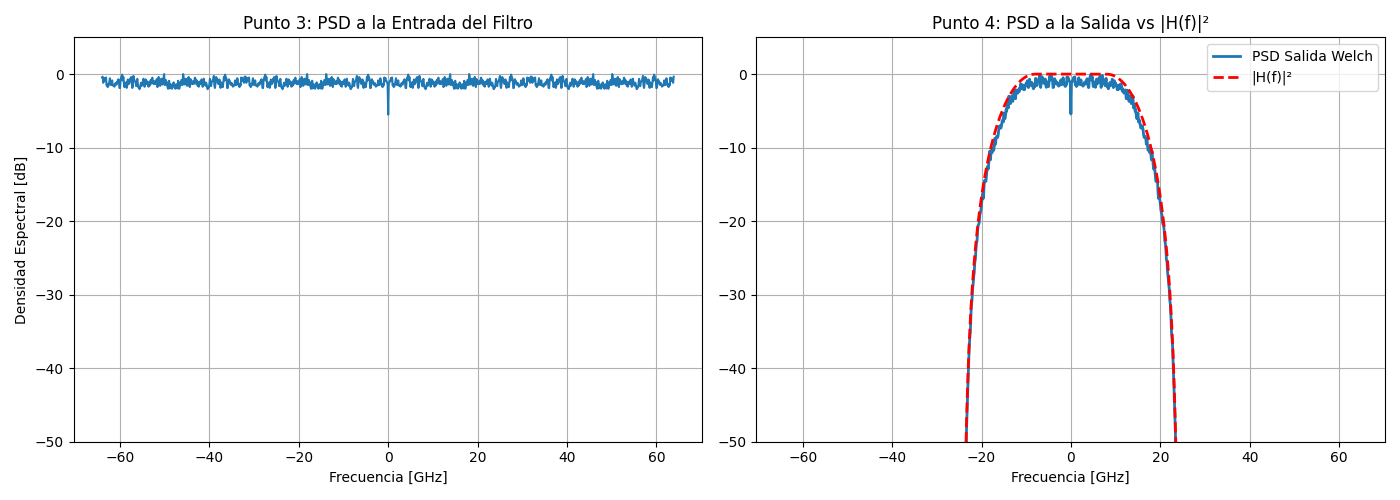
\includegraphics[width=1\linewidth]{Figura 8.png}
    \caption{\textit{PSD} a la entrada y a la salida del filtro.} 
    \label{fig:fig_8}
\end{figure}

En primer lugar, se calculó la \textit{PSD} a la entrada del filtro conformador (ver la gráfica izquierda de la \autoref{fig:fig_8}). Dado que los símbolos generados $a_{k}$ son variables aleatorias independientes e idénticamente distribuidas, la secuencia se comporta como un proceso de ruido blanco. Consecuentemente, su espectro de potencia resulta ser aproximadamente plano y constante en toda la banda de análisis.

Al analizar la señal a la salida del filtro \textit{RC} (ver la gráfica derecha de la \autoref{fig:fig_8}), se observa que la Densidad Espectral de Potencia abandona su perfil plano y adopta una morfología que calza perfectamente con la envolvente teórica del filtro elevada al cuadrado, es decir, $|H(\omega)|^{2}$. Este resultado valida la teoría de procesos estocásticos que establece que, al hacer pasar un proceso aleatorio blanco por un Sistema Lineal e Invariante en el Tiempo (\textit{SLIT}), la densidad espectral de la señal de salida queda estrictamente moldeada por la magnitud al cuadrado de la respuesta en frecuencia del sistema.




\subsection{Análisis del Sistema de Transmisión \textit{QAM-M} y Desempeño frente a Ruido \textit{AWGN}}   \label{sec_2.4}
En esta sección se analizan los resultados obtenidos de la simulación en \textit{Python} \cite{b4} de la cadena de transmisión y recepción completa para un sistema \textit{M-QAM}, utilizando filtros raíz coseno realzado (\textit{RRC}) y operando sobre un canal con ruido aditivo blanco gaussiano (\textit{AWGN}).


\subsubsection{Conformación de Pulsos y Diagrama de Ojo}            \label{sec_2.4.1}
Para limitar el ancho de banda de la señal transmitida sin introducir Interferencia Entre Símbolos (\textit{ISI}), se implementó un filtro conformador \textit{RRC} en el transmisor. En la \autoref{fig:fig_9}, se observa el diagrama de ojo a la salida del transmisor (fase en fase o parte real).
\begin{figure}[H]
    \centering
    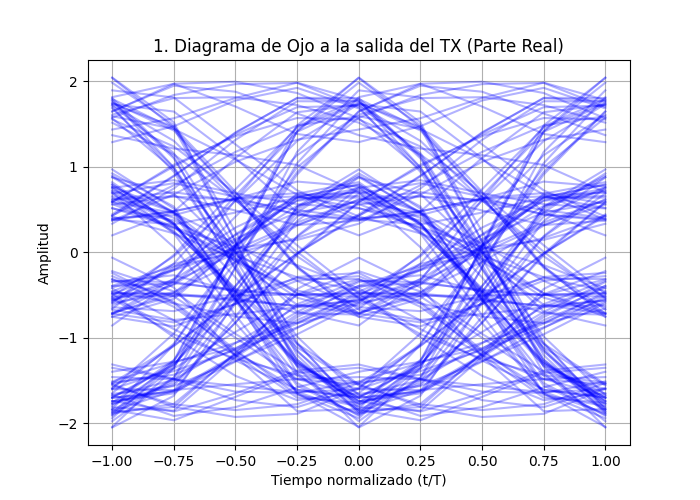
\includegraphics[width=0.65\linewidth]{Figura 9.png}
    \caption{Diagrama de Ojo a la salida del \textit{Tx}.} 
    \label{fig:fig_9}
\end{figure}

Si bien las trayectorias de la señal fluctúan debido a la memoria del filtro \textit{RRC}, el ojo se encuentra máxima y nítidamente abierto en los instantes óptimos de muestreo (centro del ojo). Esto corrobora que la combinación del filtro \textit{RRC} en transmisión con el filtro apareado \textit{RRC} en recepción logra una respuesta global de Coseno Realzado (\textit{RC}), satisfaciendo el primer criterio de \textit{Nyquist} y garantizando una transmisión libre de \textit{ISI} en el instante de decisión.


\subsubsection{Análisis Espectral (\textit{PSD})}                   \label{sec_2.4.2}
El efecto del filtrado y del canal puede observarse claramente en el dominio de la frecuencia. En la \autoref{fig:fig_10}, se compara la Densidad Espectral de Potencia (\textit{PSD}) de la señal transmitida con la señal a la entrada del receptor.
\begin{figure}[H]
    \centering
    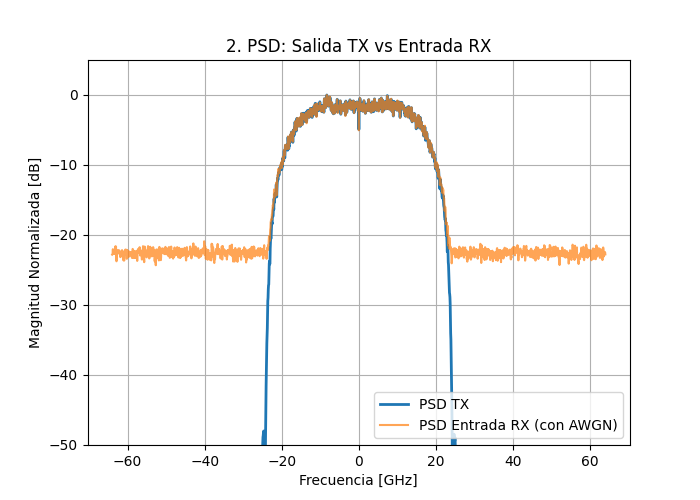
\includegraphics[width=0.7\linewidth]{Figura 10.png}
    \caption{\textit{PSD} Salida \textit{Tx} vs Entrada \textit{Rx}.} 
    \label{fig:fig_10}
\end{figure}

Se aprecia cómo el canal \textit{AWGN} eleva el piso de ruido de la señal recibida. Posteriormente, la señal ingresa al filtro apareado en el receptor. La \autoref{fig:fig_11} ilustra la acción de este filtro.
\begin{figure}[H]
    \centering
    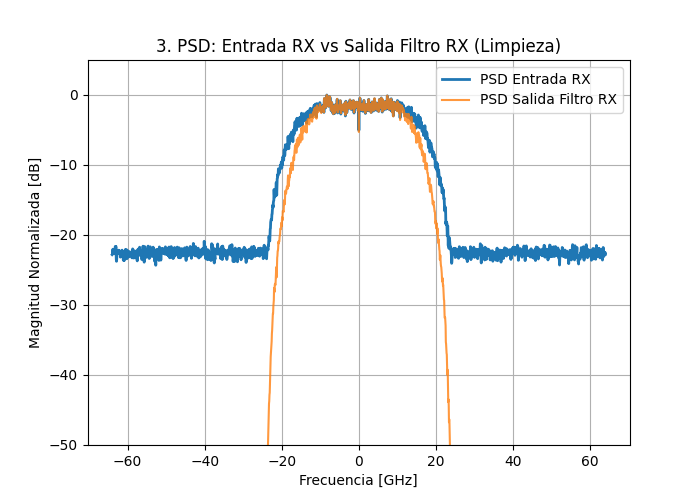
\includegraphics[width=0.7\linewidth]{Figura 11.png}
    \caption{\textit{PSD} Entrada \textit{Rx} vs Salida Filtro \textit{Rx}.} 
    \label{fig:fig_11}
\end{figure}

El filtro apareado cumple un doble propósito: por un lado, completa el filtrado \textit{RC} para anular la \textit{ISI}; por el otro, rechaza el ruido fuera de la banda de interés, maximizando así la Relación Señal a Ruido (\textit{SNR}) antes de la etapa de decisión.


\subsubsection{Constelación y Distribución del Ruido}               \label{sec_2.4.3}
Tras el filtrado apareado y la correcta alineación temporal para compensar el retardo de los filtros, las muestras ingresan al \textit{slicer}. La \autoref{fig:fig_12} muestra la constelación recibida para un $E_{b}/N_{0}$ de $15 \ [dB]$ en una modulación \textit{QAM-16}.
\begin{figure}[H]
    \centering
    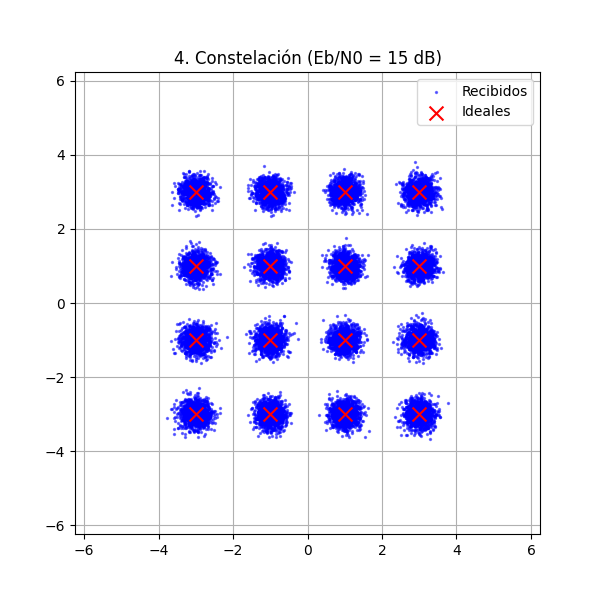
\includegraphics[width=0.6\linewidth]{Figura 12.png}
    \caption{Diagrama de Constelación para \textit{QAM-16} con $E_{b}/N_{0} = 15 \ [dB]$.} 
    \label{fig:fig_12}
\end{figure}
\begin{figure}[H]
    \centering
    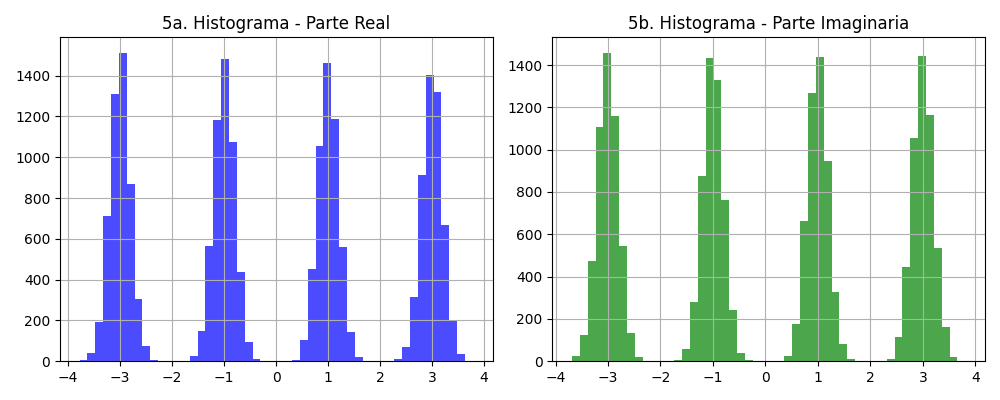
\includegraphics[width=1\linewidth]{Figura 13.png}
    \caption{Histograma de parte real e imaginaria para \textit{QAM-16}.} 
    \label{fig:fig_13}
\end{figure}

Los símbolos recibidos (dispersos en azul) se agrupan alrededor de los símbolos ideales (cruces rojas). La dispersión observada es producto exclusivo del ruido térmico (AWGN), ya que la ISI ha sido mitigada. Como se corrobora en los histogramas de las componentes en fase y cuadratura, esta dispersión sigue una distribución netamente gaussiana.


\subsubsection{Análisis de la Tasa de Error de Bit (\textit{BER})}  \label{sec_2.4.4}
Finalmente, para cuantificar la robustez del sistema, se simuló la probabilidad de error variando la relación $E_{b}/N_{0}$. En la \autoref{fig:fig_14}, se contrastan las curvas de \textit{BER} simuladas frente a las teóricas para modulaciones \textit{QPSK} y \textit{QAM-16}.
\begin{figure}[H]
    \centering
    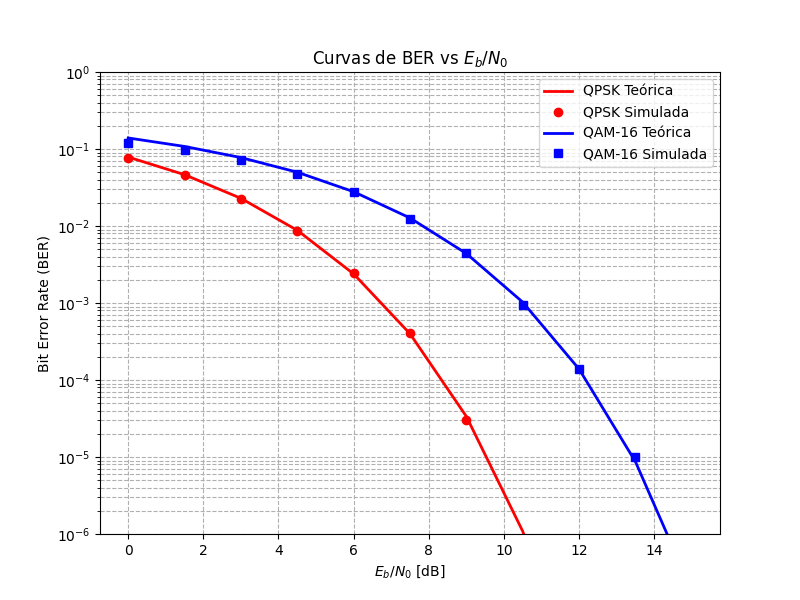
\includegraphics[width=0.8\linewidth]{Figura 14.png}
    \caption{Curvas de \textit{BER} vs $E_{b}/N_{0}$ para \textit{QPSK} y \textit{QAM-16}.} 
    \label{fig:fig_14}
\end{figure}

Los resultados de la simulación tienen un ajuste casi perfecto con las expresiones teóricas en todo el rango evaluado (hasta un \textit{BER} del orden de $10^{-6}$). Como era de esperarse, la modulación \textit{QAM} requiere un mayor $E_{b}/N_{0}$ ($\approx 4 \ [dB]$ adicionales) en comparación con \textit{QPSK} para mantener la misma tasa de error, evidenciando el compromiso fundamental entre eficiencia espectral y robustez frente al ruido.




\section{Conclusiones}                                              \label{sec_3}
El desarrollo de este trabajo práctico permitió validar mediante simulación computacional la cadena completa de transmisión y recepción de un sistema \textit{QAM-M}. Se comprobó empíricamente la importancia crítica de utilizar filtros apareados Raíz de Coseno Realzado (\textit{RRC}), los cuales demostraron ser altamente efectivos para limitar el ancho de banda, maximizar la relación señal a ruido y anular la Interferencia Entre Símbolos (\textit{ISI}) en los instantes óptimos de muestreo.

Por otro lado, el análisis de desempeño frente a un canal con ruido aditivo (\textit{AWGN}) arrojó resultados concluyentes, logrando curvas de Tasa de Error de Bit (\textit{BER}) que calcan las expresiones teóricas con extrema precisión. Esto no solo valida la robustez del simulador desarrollado, sino que evidencia el compromiso fundamental de estos sistemas: incrementar la eficiencia espectral (como al transicionar de \textit{QPSK} a \textit{QAM-16}) exige invariablemente un aumento en la energía de bit ($E_{b}/N_{0}$) para mantener la confiabilidad del enlace.


\newpage
\printbibliography[heading=bibintoc, title={4. \ Bibliografía}]

\end{document}